\infolevone{

\section{Old Beamline stuff}

[From the old Hall C manual.  Move info here into above sections as needed.]

It executes the following functions:

\begin{itemize}
\item{Provide a fine waist focusing on the target.}
\item{Beam energy, beam energy spread, and beam emittance measurements
in the arc section.}
\item{Vertical chicane beam transfer for the polarized target.}

\item{High precision beam angle measurement for selected cross section
experiments.}
\end{itemize}

\subsection{Control}

All magnets (dipoles, quads, sextupoles, beam
correctors) and beam diagnostic devices (BPM, harp, BCM, viewer)
are controlled by machine control center (MCC) through EPICS,
except for a few special elements, which are addressed in the
subsequent Sections.

\subsection{Monitoring}
To start up the beam position monitor (BPM) and beam current monitor
(BCM) displays which are normally displayed continuously on X-terminal
HALLCXT9, do these steps:
\begin{itemize}
  \item {as cvxwrks on cdaqh1, run \texttt{medm}.}
  \item {click \texttt{execute}.}
  \item {{\em For BPM}open \texttt{MEDM/bpm/gueye/hcbpms\_gueye\_jan99.adl}}
  \item {{\em For BCM}open \texttt{MEDM/saw/bcm.adl}}
\end{itemize}

\subsection{Safety procedures}

Detailed safety procedures are specified in the following documents:

\begin{itemize}
\item{Fast shut down system}
\item{MCC emergency plan}
\item{Incident-response procedure}
\item{Safety systems reference and procedure}
%\item{Search and secure procedure}
%\item{Electrical-hazard testing procedure}
%\item{Entry requirements}
%\item{Safety inspection checklists}
%\item{PSS interlock}
%\item{Radiation exposure emergency response procedure}
\end{itemize}

\subsection{Machine/Beam line protection system}

The MPS system is composed of the fast shutdown (FSD), beam loss
monitor (BLM), beam loss accounting (BLA), and gun control systems.

The FSD system is a network of permissive signals which terminate
at the electron gun. The permissive to the gun may be inhibited by any 
device connected to an FSD node.
Devices connected to the FSD system include vacuum valves, RF
systems, beam loss systems, beam current monitors, and beam dumps.

The gun control system includes software program which monitor
beam operating conditions and the state of the FSD, BLM, and BLA systems.
The program will warn the operators if a potential for beam damage
exists. Potential for damage exists when running high average current
beam, when FSD nodes are masked, and when the beam power approaches
the operating envelope limits for a specific beam dump.

\subsection{Reference documents}

The following Reference Documents are available:

\begin{itemize}
\item{Accelerator Operations Directives, May 9, 1994}
\item{Tunnel song sheet and drawings, June 25, 1995}
\item{Hall~C beam line elements list, June 9, 1994}
\item{Hall~C team summary notebook}
\item{Hall~C beam line commissioning procedure, May 1995}
\item{Hall~C beam energy measurement commissioning procedure, June 22, 1995}
\end{itemize}

\section{Special Beam Line Elements}

There are several special beam line elements which were temporarily
controlled by the Hall~C group. We transfered them to machine
control center in 1996 when the R\&D period was over.

Those special beam line elements include:  raster systems; superharp systems; the M\o ller 
Polarimeter; the bremsstralung radiator; and current measuring devices.

\subsection{Superharp Systems}

The superharp systems are mainly used for beam energy measurement,
but are also used as a reference for BPM calibration, and as
normal beam profile monitors for machine operation. Three pairs
of superharps are located on the pre-aligned granite tables at the
beginning, the mid-point, and the end of arc.
Separate superharps are located in combination with BPM's in the
Hall~C beamline segment close to the Hall~C target.

When the Hall~C arc is tuned in the so-called ``dispersive" mode
the three pairs of superharps are successively operated to obtain
the positions and orientations of the incident and outgoing beam,
which renders also the central trajectory. The combination of
beam positions and beam profile as given by the three superharp
pairs, together with the known field integral of the arc bend
magnets, can be used to derive the beam energy and also the beam
emittance and dispersion.

Anyone who has access to enter the Hall~C beam line tunnel should
not bump the three granite tables because the superharp
crosses are aligned with high precision. Any beam line work in this
section should be discussed with the JLab survey group in advance.

Superharp operation is shared by Hall~C and MCC. To prevent any
disturbance of software an authorized path and area must be
installed for its secure operation. Anyone (including Hall~C persons
and users) who wants to change directory or reboot IOC should
report to the responsible personnel
in advance.

With the normal scan velocity setting of 20000 Steps per second, the
maximum cw current that the 22 micron tungsten wire can stand is about
20 $\mu$A. Above this value superharp operation is prohibited.

The following Reference Documents are available:
\begin{itemize}
\item{JLab-R-94-01}
\item{JLab HARP record detailed design document, D. Barker, May 31, 1994}
\item{Hall~C requirements for the superharp scanning system, D.
Barker, C. Yan}
\end{itemize}


\paragraph{The Superharp Device}\label{system}

The superharp consists of a wood fork holding a 22~$\mu$m tungsten wire segmented in three
perpendicular sections. This fork can be inserted in and out of the beam pipe, causing an
interaction between the wires and the electron beam (Fig.~\ref{figure:superharp}).


\begin{figure}[!hbt]
\begin{center}
%\htmlimage{flip=r270}
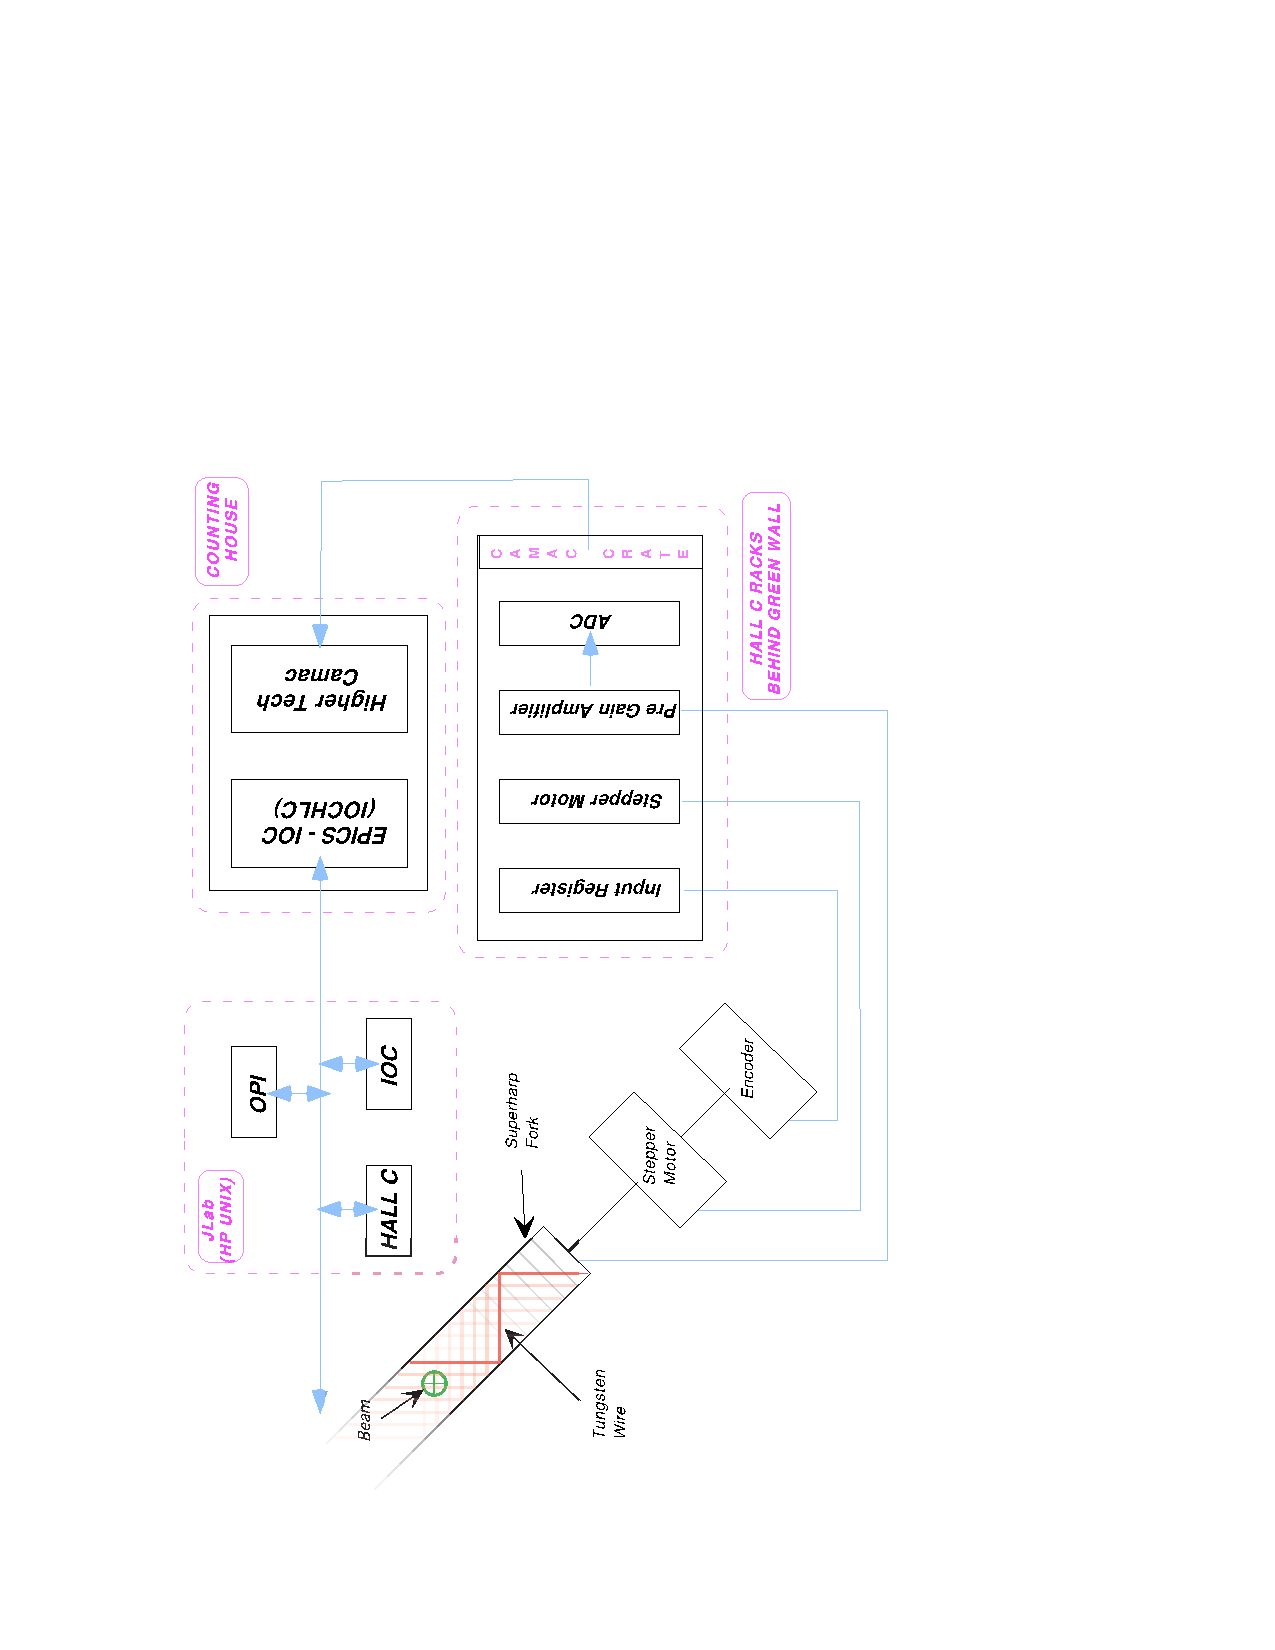
\includegraphics[width=6in,angle=270]{superharp-system.pdf}
\caption{Schematic of the superharp system.}
\label{figure:superharp}
\end{center}
\end{figure}

The horizontal and vertical positions of the beam are then determined by collecting the charges
produced as the wires go through the electron beam within an accuracy of about 
%!!! $\pm 50~\mu$m
(see Fig.~\ref{figure:interface} in section~\ref{interface}). While the superharp fork
is travelling inside the beam pipe, three diferent signals appears due to the interaction
between the JLab beam and each of the three wires. The time duration during a scan is
approximately 30~sec from the starting rest position to the maximum allowed travel distance
(about 3''=7.62~cm).

The signals are then sent to an Analog Digital Converter (1881-ADC) electronic card and then transfered
to a computer for data analysis. Due to the interaction beam-wires, this device spreads the beam
(destructive method). In addition, with the information on the horizontal position inside the arc, the
energy of the electron beam can also be monitored~\cite{Gueye-98-energy}. This feature will be described
later in section~\ref{analysis}. The current range for these wires is
between 1 and 30~$\mu$A.  

Since some experiments in hall C will run with a current below
1~$\mu$A,  some BLMs have been added to the
current electrode channels.

The Beam Loss Monitor (BLM) is a photo-multiplier tube (Hamamatsu-931B, side cathode) which detects
particles produced when the wires from the superharp's fork interacts
with the  electron beam. Each
superharp has one BLM located downstream about 10~cm (target) and
0.5-2~m ( hall C arc). Combined with
the electrode channel, the total current range of a single superharp device is
$0.01 < I~(\mu {\rm A}) < 30$.

\paragraph{The superharp interface window}\label{interface}

The automated hall C superharp interface window program allows control of both
data acquisition and data analysis. The flow chart of the code is shown on Fig.~\ref{figure:flow_chart}. 
Each superharp device is controlled via 
\htmladdnormallinkfoot{EPICS}{http://epics.aps.anl.gov/asd/controls}. The
signals obtained from a scan are then
stored into an ASCII file which serves as an input file for a {\tt C++} routine where all the
calculations are performed. The main interface window is shown on Fig.~\ref{figure:interface}.

\begin{figure}[!hbt]
\begin{center}
%\htmlimage{thumbnail=0.5,scale=1.0}
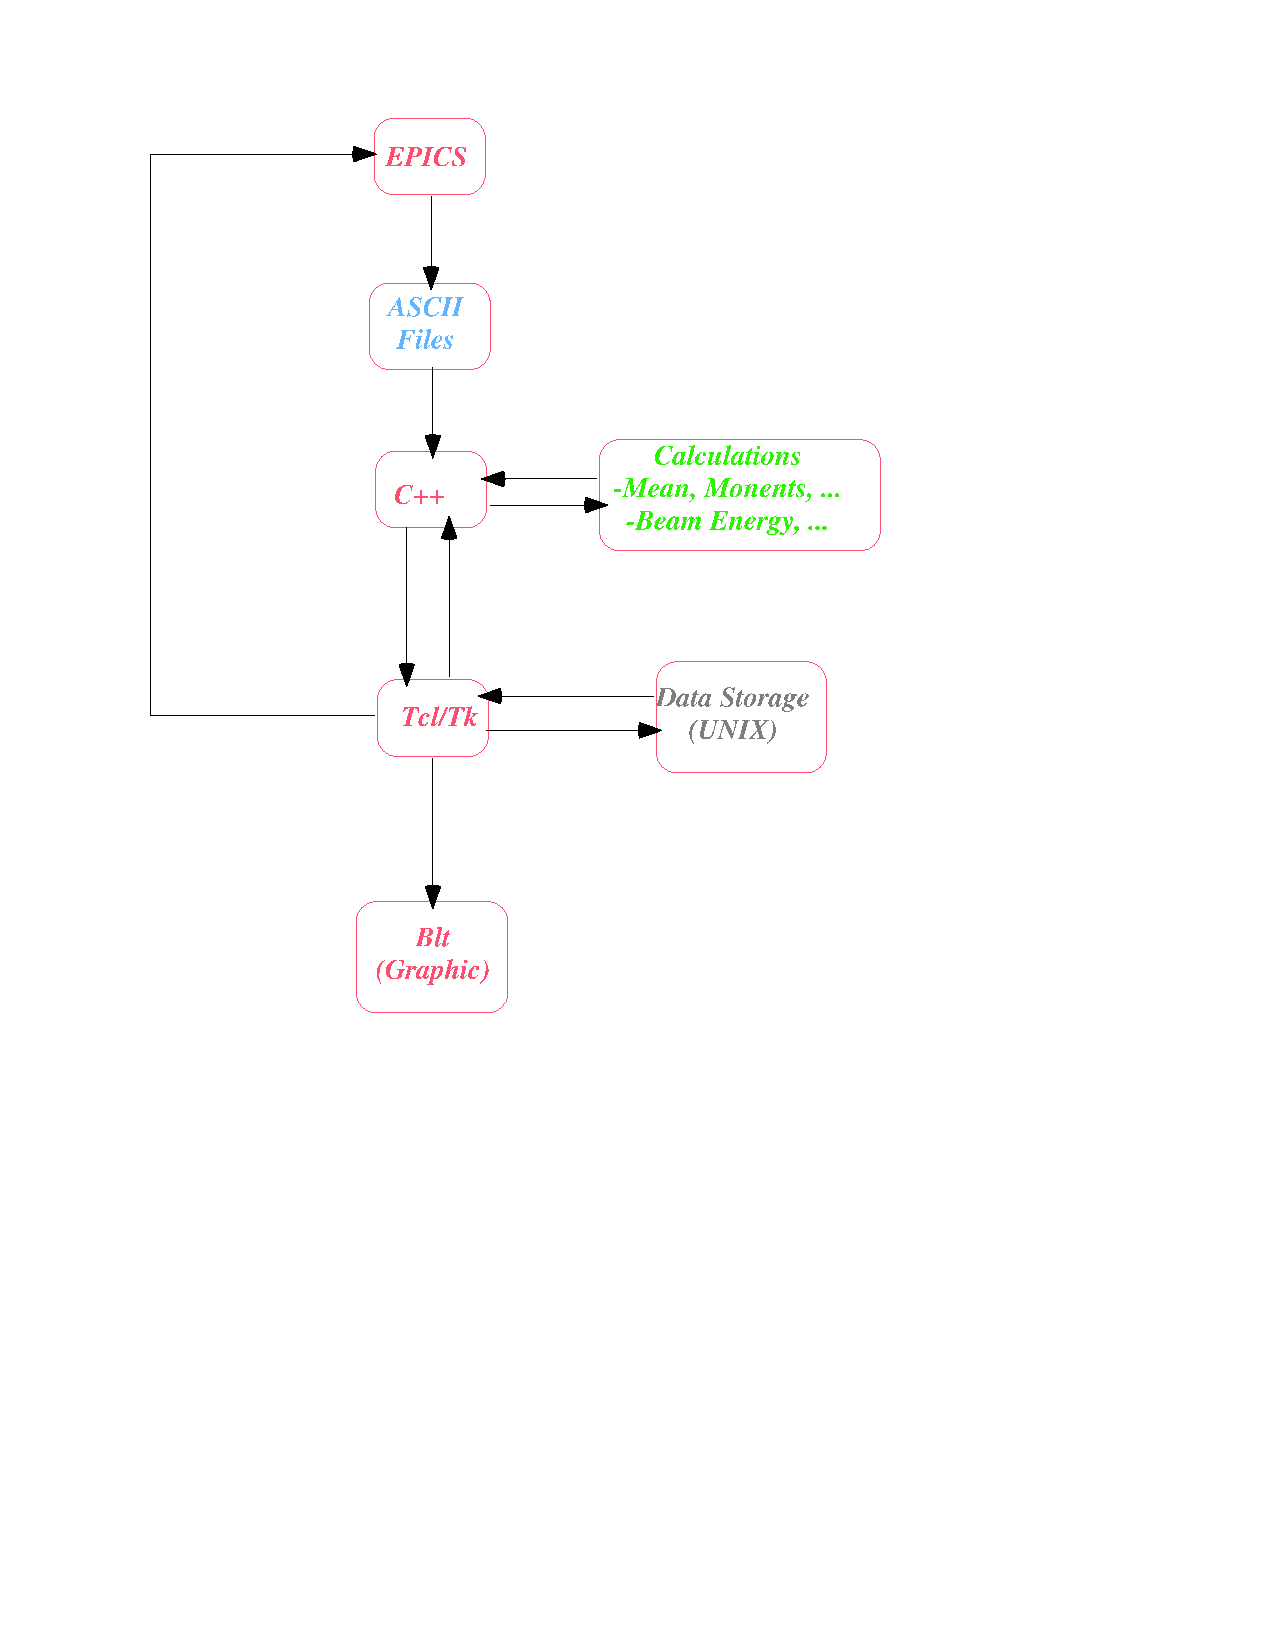
\includegraphics{superharp-flowchart.pdf}
\caption{Flowchart of the hall C superharp interface program.}\label{figure:flow_chart}
\end{center}
\end{figure}

%%note: natural size of following figure is 7wx8.85h inches.
\begin{figure}[!hbt]
\begin{center}
%\htmlimage{thumbnail=0.5,scale=4.0,flip=r270}
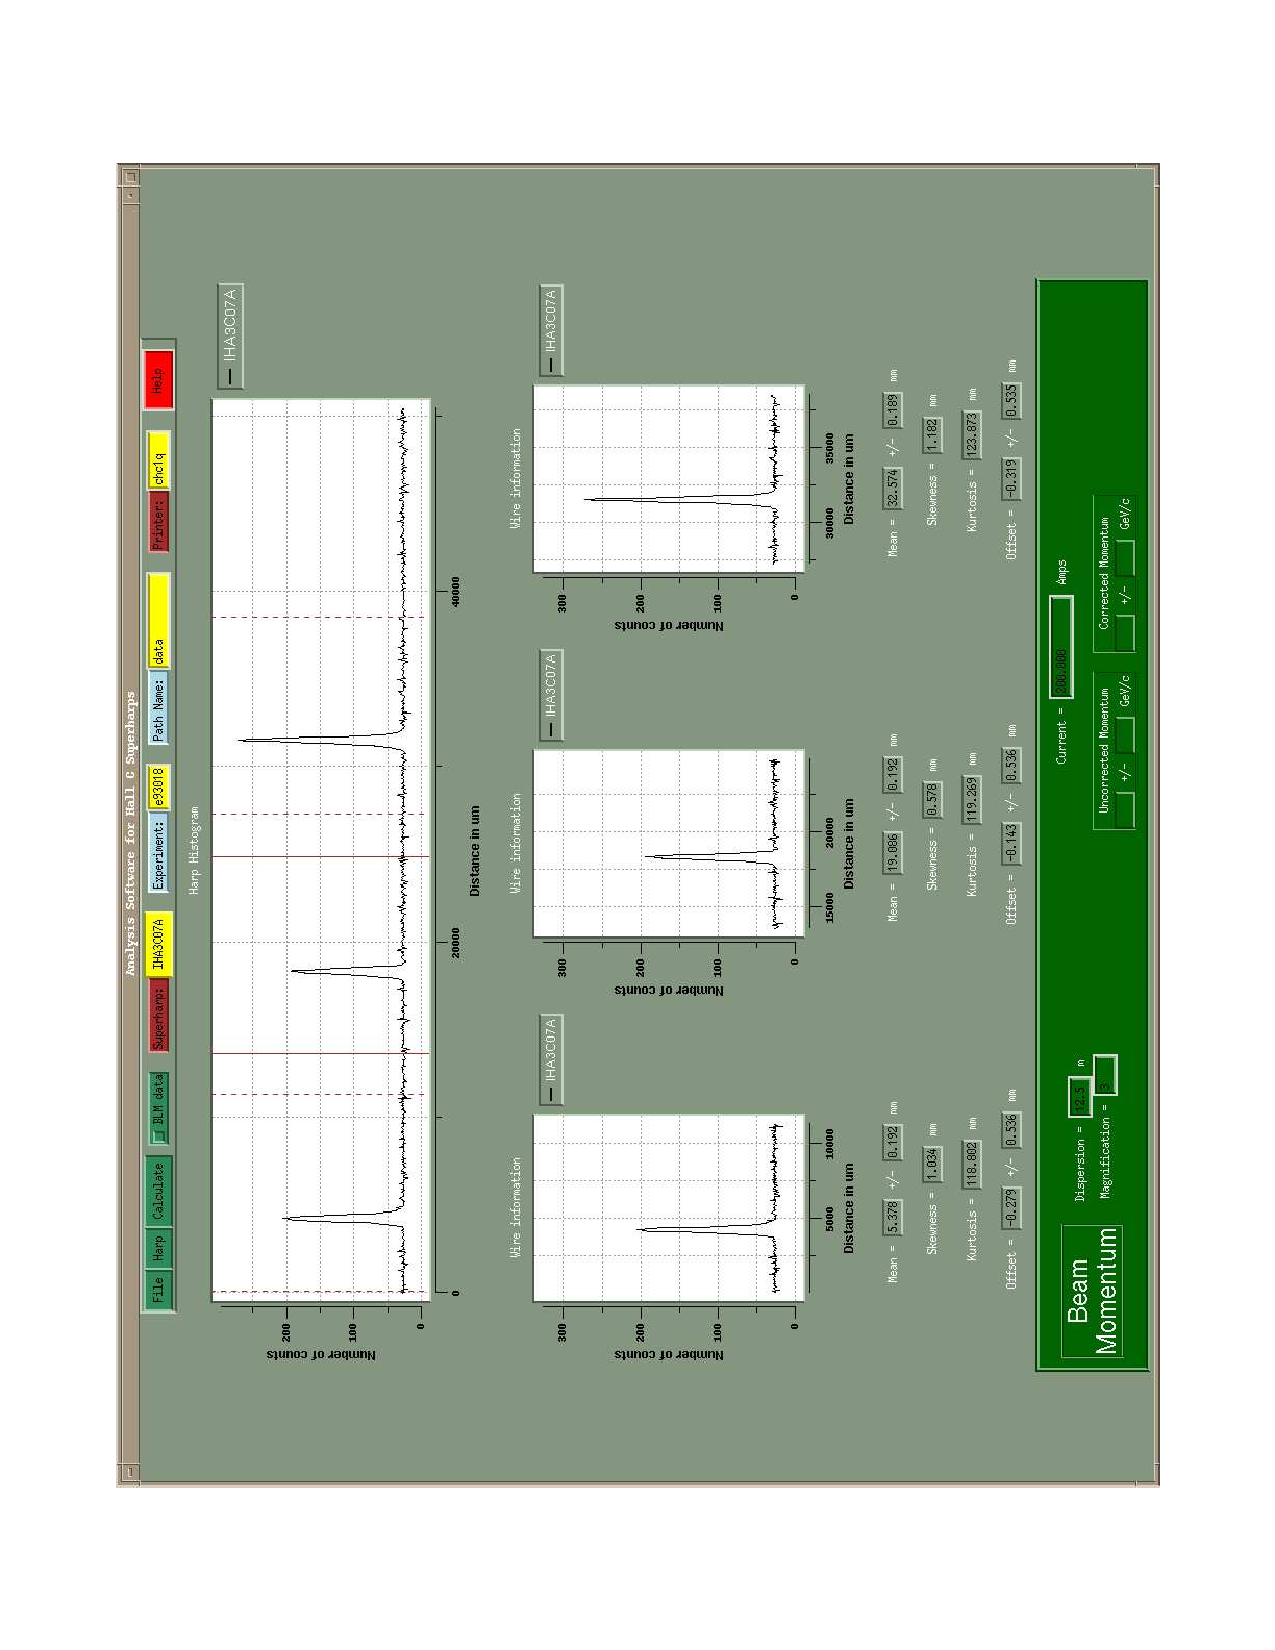
\includegraphics[height=6.5in,width=5.5in]{superharp_interface.pdf}
\caption{The hall C superharp interface window.}\label{figure:interface}
\end{center}
\end{figure}

In this section, we will review the different menu items that allow users to perform a scan and
perform data analysis.

	\subparagraph{Data Acquisition}\label{daq}

The corresponding code is running only on the actual {\bf cdaqh1} cluster located in the experimental
hall C counting house. Selecting {\bf\fbox{Harp $>$ Scan}} launches the {\tt MEDM} executable routine.

There are two control panels: one allows the user to select the appropriate superharp
(Fig.~\ref{figure:choose_harp}) and one to perform the scanning process (Fig.~\ref{figure:scan_harp}).

\begin{figure}[!hbt]
\begin{center}
%\htmlimage{thumbnail=0.5,scale=2.0}
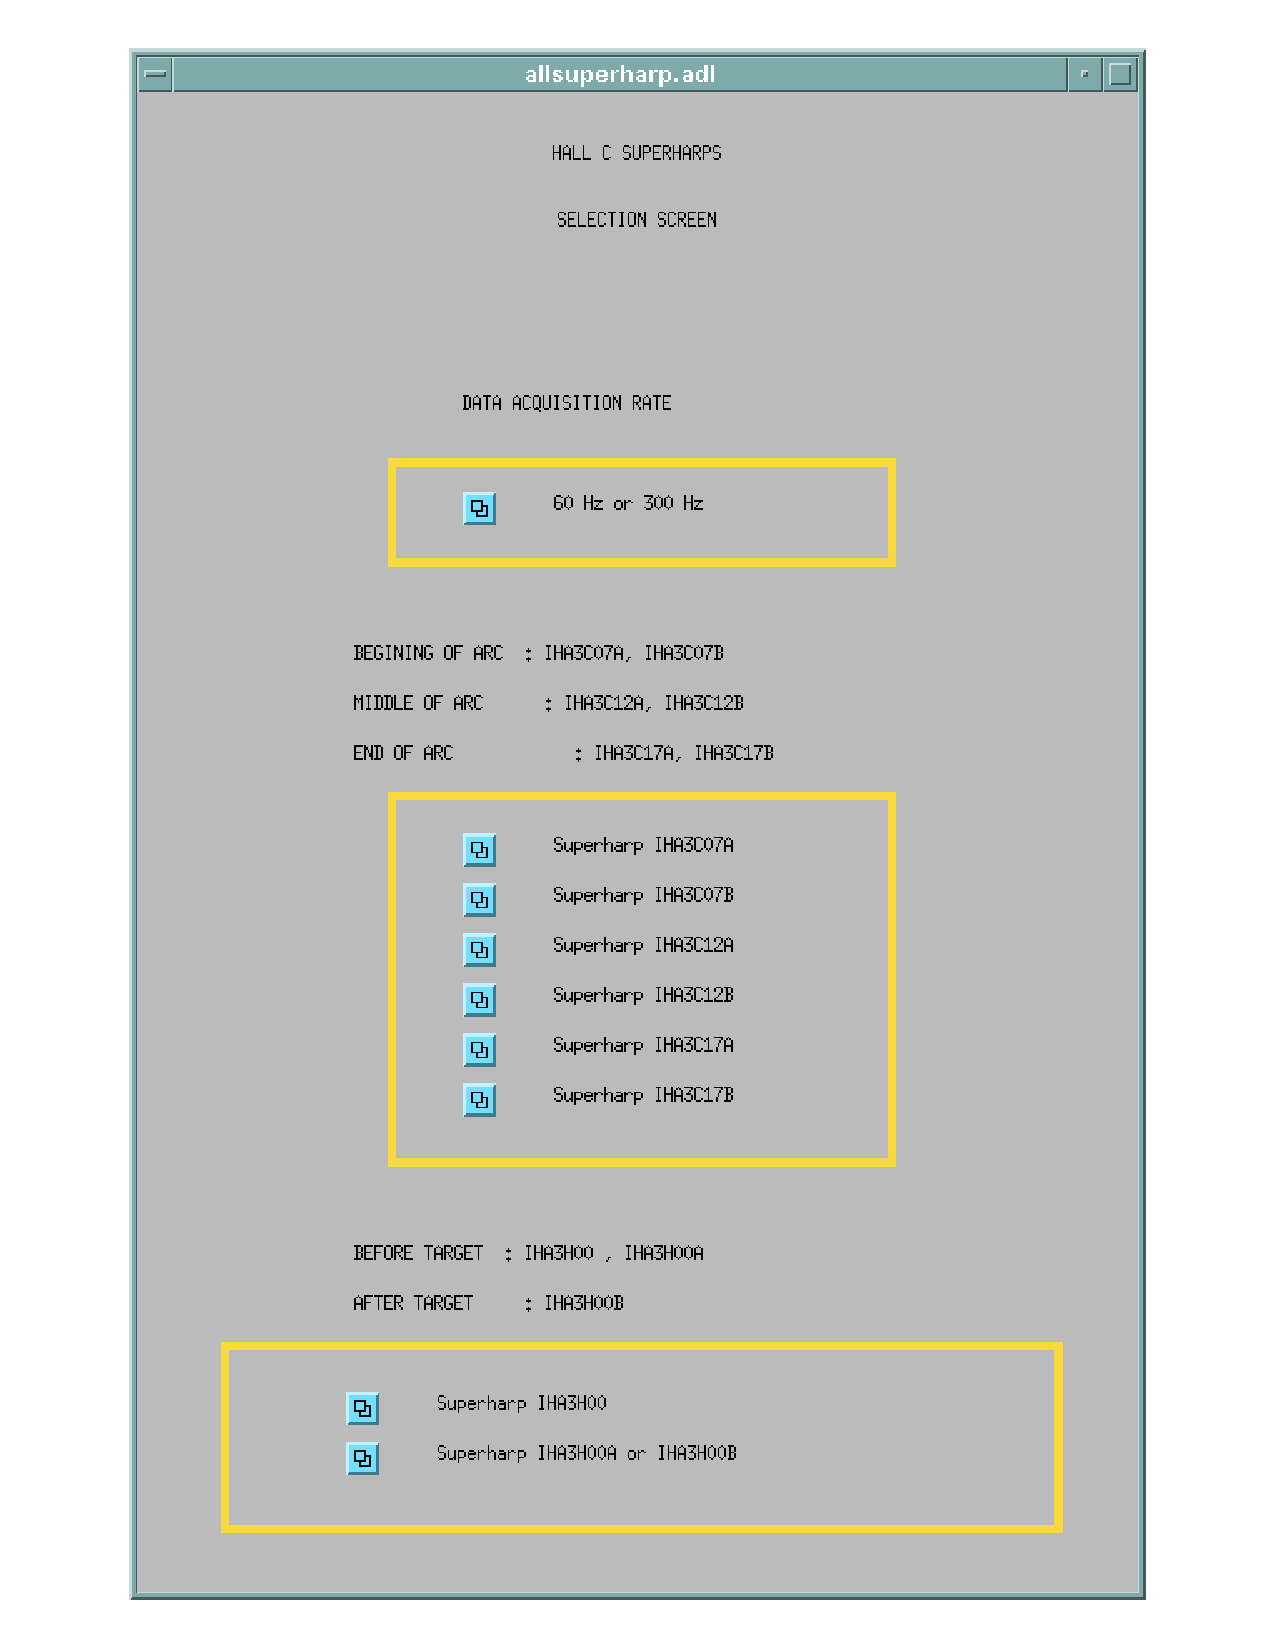
\includegraphics[height=7.2in]{superharpChoicePanel.pdf}
\caption{The hall C superharp selection control panel.}\label{figure:choose_harp}
\end{center}
\end{figure}


\begin{figure}[!hbt]
\begin{center}
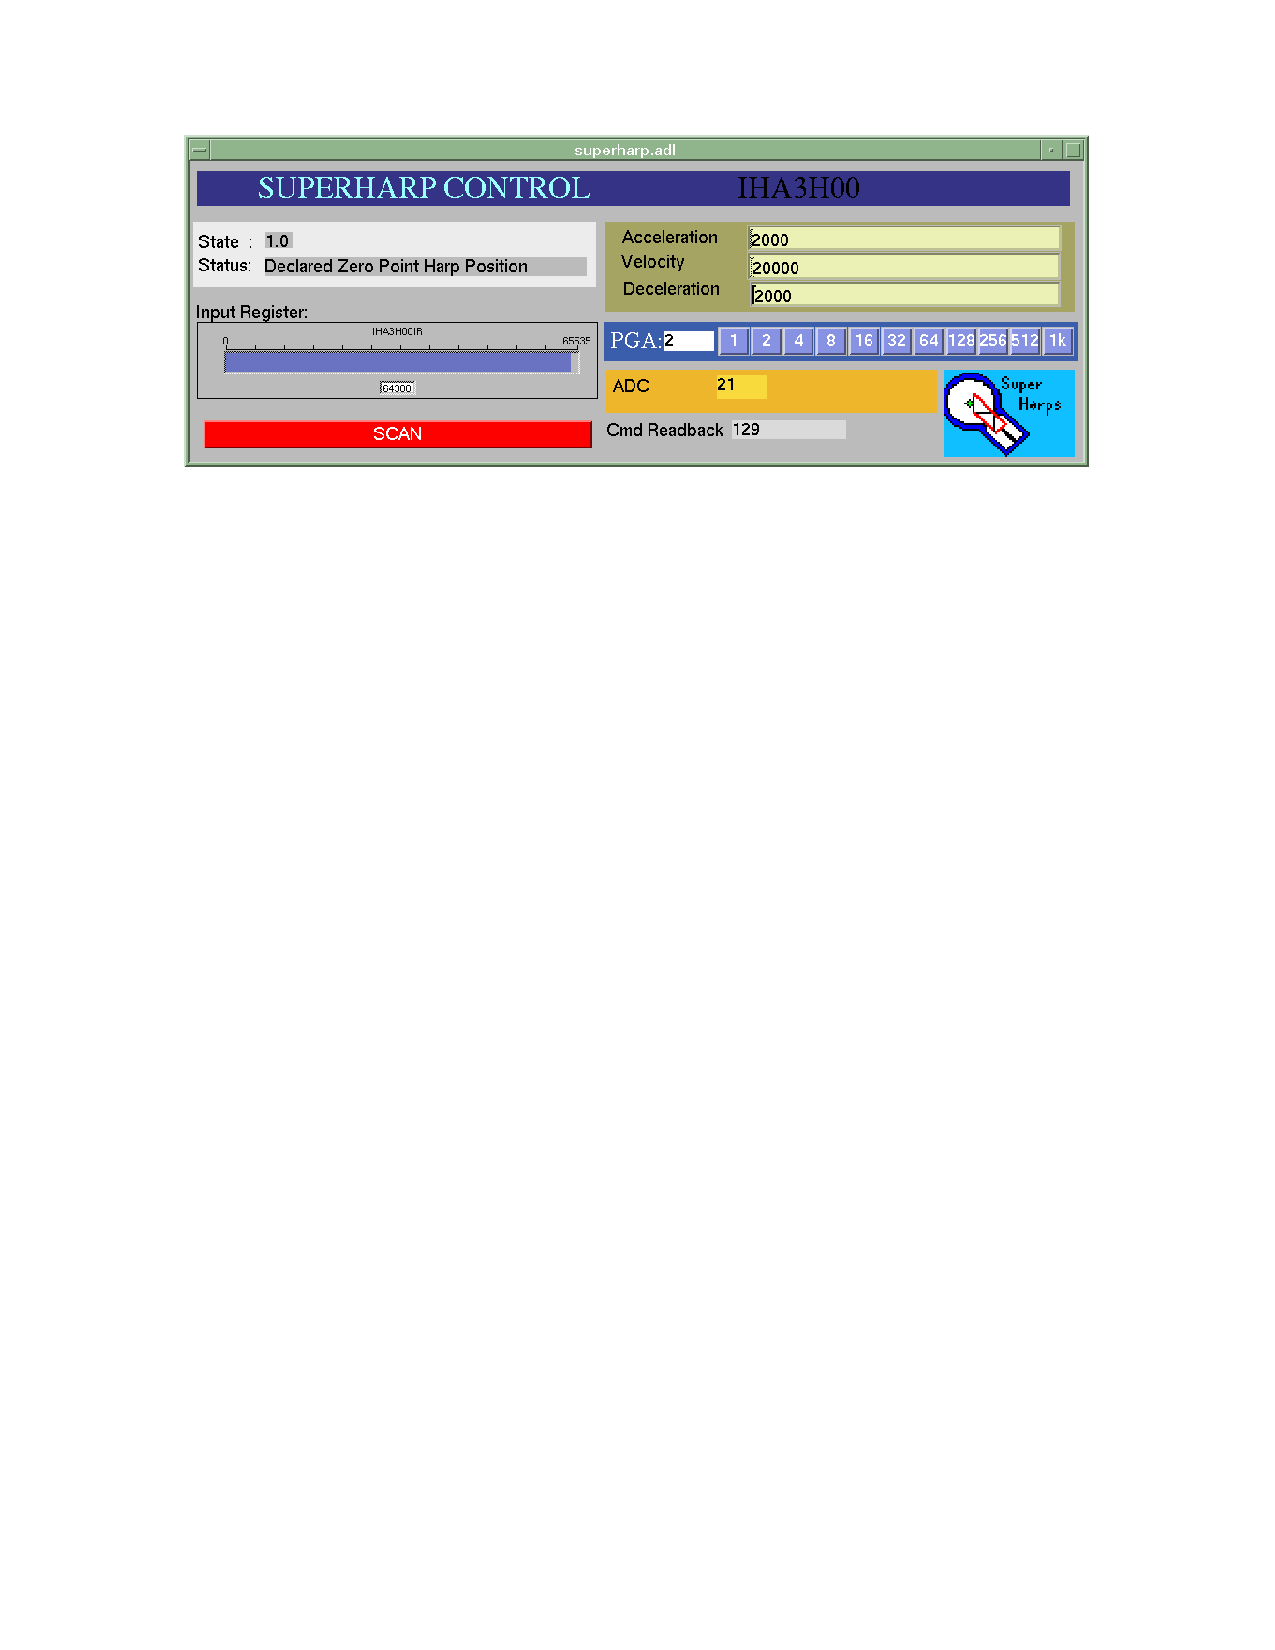
\includegraphics{scan-panel.pdf}
\caption{The hall C superharp scanning control panel.}\label{figure:scan_harp}
\end{center}
\end{figure}

Before starting any scanning process, verify that you have the correct default parameters as shown in
Table~\ref{table:scan_harp} below.
\begin{table}[!hbt]
\begin{center}
\begin{tabular}{llr}
\hline
\hline
{\it Values:}			&	\\ 
Acceleration			& 2000~tr/min	\\
Velocity			& 20000~tr/min	\\
Deceleration			& 2000~tr/min	\\
Pre-Gain Amplifier (PGA)	& 2	\\
\hline
\hline
{\it Messages:} 		&	\\
State				& 1	\\
Status				& Declared Zero Point Harp Position \\
Input Register			& 64335 \\
Analog Digital Converter (ADC) counts& 10-30 (background) \\
Cmd Readback			& 129	\\
\hline
\hline
\end{tabular}
	\caption{The default scan parameters for the hall C superharp system.}
	\label{table:scan_harp}
\end{center}
\end{table}
If not, then enter the correct value(s) and hit {\bf\fbox{return}}. Note that the value will {\bf not}
change  unless you hit \fbox{\bf return}. The last two digits in the
{\bf\fbox{Input Register}} box may
not be the same due to the 10~$\mu$m accuracy of the encoder.

After launching {\tt MEDM}, click on the red {\bf\fbox{SCAN}} button to begin the scan. The list
below describes the  change in several important variables during the scanning process.
\begin{enumerate}
\item \fbox{{\bf State}} changes from 1 to 4.
\item \fbox{{\bf Status}} indicates {\it Harp is moving}, {\it Harp is retracting}, and
	{\it Declared zero harp position} during the corresponding motion of the harp.
	{\it Declared zero harp position} indicates that the scan is finished and the harp has
	returned to its fully retracted rest position.
\item \fbox{{\bf Velocity}} changes to 30000~tr/min when the harp comes back.
\item \fbox{{\bf ADC}} registers the number of electrons picked up when a wire crosses the beam.
\item \fbox{{\bf Cmd Readback}} reads {\bf 66} when the harp is moving in the forward direction
	and {\bf 65} in the backward direction.
\end{enumerate}


	\subparagraph{Data analysis}\label{analysis}

Although \fbox{\bf harp\_ana\_new} is the main executable, the files \fbox{\bf harp\_ana\_new.tk}
and \fbox{\tt bltwish} are both required: \fbox{\bf  harp\_ana\_new.tk} contains the graphical routines
for the program and is interpreted at run-time through \fbox{\bf bltwish}. \fbox{\bf harp\_ana\_new} contains
both {\tt C++} and {\tt Tcl/Tk} codes: \fbox{\bf harp\_ana\_new} is written in {\tt C++} and contains most
of the calculation routines, and \fbox{\bf  harp\_ana\_new.tk} is written in {\tt Tk} and contains the user
interface and graphing routines.

	\subparagraph{Menu and entry Items}

The menu commands and entry items are described in Table~\ref{table:menu_entry}.
\begin{table}
\begin{center}
\begin{tabular}{||l|c|l||}
\hline
\hline
\multicolumn{3}{|c|}{\bf Menu Commands and Accelerator}	\\
\hline
File Reset & Ctrl-R & Clears all graphs and removes all data. \\
File Load  & Ctrl-L & Load all data in the current path. \\
File Save  & Ctrl-S & Saves all data in the current path. \\
File Print & Ctrl-P & Prints all graphs to the current printer.\\
File Quit & Ctrl-Q & Exits the program. \\
\hline
Harp Options & & Calls the configuration dialog. \\
Harp Scan & & Launches the medm scanning routine. \\
\hline
Calculate dP/P0 & & Calculates $P$ and $\Delta P$ based on the current data. \\
Calculate Smooth & Ctrl-M & Filters out background noise in all graphs. \\
Calculate Unsmooth & Ctrl-U & Reverses Calculate Smooth. \\
Calculate Transform & Ctrl-T & Calculates the Fourier cosine transform \\
		& & of the data. \\
\hline
\hline
\multicolumn{3}{|c|}{\bf Entry Items}	\\
\hline
Superharp	& & Load the selected superharp from the path	\\
		& & listed in the {\it File Name} entry and graphs it		\\
Experiment	& & Specifies the number of the current experiment.	\\
		& & The destination for files created by File Save 	\\
		& & is {\tt scan\_data/}{\it{Experiment}}{\tt /}{\it File Name}	\\
File Name	& & Specifies the location of the harps to be loaded	\\
		& & or the destination for the files created			\\
		& & by File Save			\\
Printer		& & Specifies the current printer				\\
\hline
\hline
\end{tabular}
	\caption{Definition of the menu commands, accelerators and entry items.}\label{table:menu_entry}
\end{center}
\end{table}

	\subparagraph{Help and BLM data}

The two remaining buttons on the superharp interface window menu bar, \fbox{{\bf BLM data}} and
\fbox{{\bf Help}}, allow users to switch to the BLM channels and displays this document ({\tt harphelp.ps}),
respectively.

\paragraph{Using the Program}\label{program}

This section describes in detail how to use harp\_ana\_new to execute common commands.

	\subparagraph{Loading Old Harp Data}

Data is loaded by selecting the name of the harp from the {\it Superharp} drop-down menu.  The program
looks in the path {\tt scan\_data/}{\it Experiment}{\tt /}{\it File Name}, where {\it Experiment} is
the experiment number listed in the {\it Experiment} entry and {\it File Name} is the file name listed
in the {\it File Name} entry.

	\subparagraph{Loading New Harp Data}

Data collected through Options Scan is automatically converted into a format readable by
{\fbox{\bf harp\_ana\_new}}, so it can been loaded, even in the same session in which it was collected,
as if it were old harp data.

	\subparagraph{Graphing Old Harp Data}

Harp data is automatically graphed when loaded (by selecting it from the {\it Superharp} drop-down menu).
The statistical information for the first graph loaded is also displayed.

	\subparagraph{Graphing New Harp Data}

Connect to {\tt cdaqh1} and run \fbox{\bf harp\_ana\_new}.  Select \fbox{Options Scan}, and follow the
instructions in the {\tt MEDM} section to scan in new data.  After exiting {\tt MEDM}, the new data should
appear. Note that it takes about 10 to 15 seconds for {\tt MEDM} to load.

	\subparagraph{Saving Harp Data}

Selecting \fbox{File Save} saves and compresses (using {\tt gzip}) the data for all the harps
currently loaded in the directory {\tt scan\_data/}{\it Experiment}{\tt /}{\it File Name}, where
{\it Experiment} is the experiment number listed in the {\it Experiment} entry and {\it File Name}
is the file name listed in the {\it File Name} entry.  If the directory {\tt scan\_data/}{\it Experiment}
does not already exist, it is automatically created.

	\subparagraph{Printing Harp Data}

Selecting \fbox{File Print} prints a screen capture to the printer listed in the {\it Printer} entry.

	\subparagraph{Removing Harp Data}

Selecting \fbox{File Reset} clears all harp data from the screen and from memory (but doesn't
erase the files from disk).


	\subparagraph{Fourier Transform}

It has been demonstrated that the JLab beam has a fundamental 60~Hz motion originating from the power
line. In order to have a precise determination of the position of the beam, correction from this beam
motion is necessary. For that purpose, a Fourier transform which returns the beam motion harmonics to
all orders from the data has been developped.

Selecting \fbox{Calculate Transform} calls the dialog box displayed in Fig~\ref{fig:transform}.
\begin{figure}[htp]
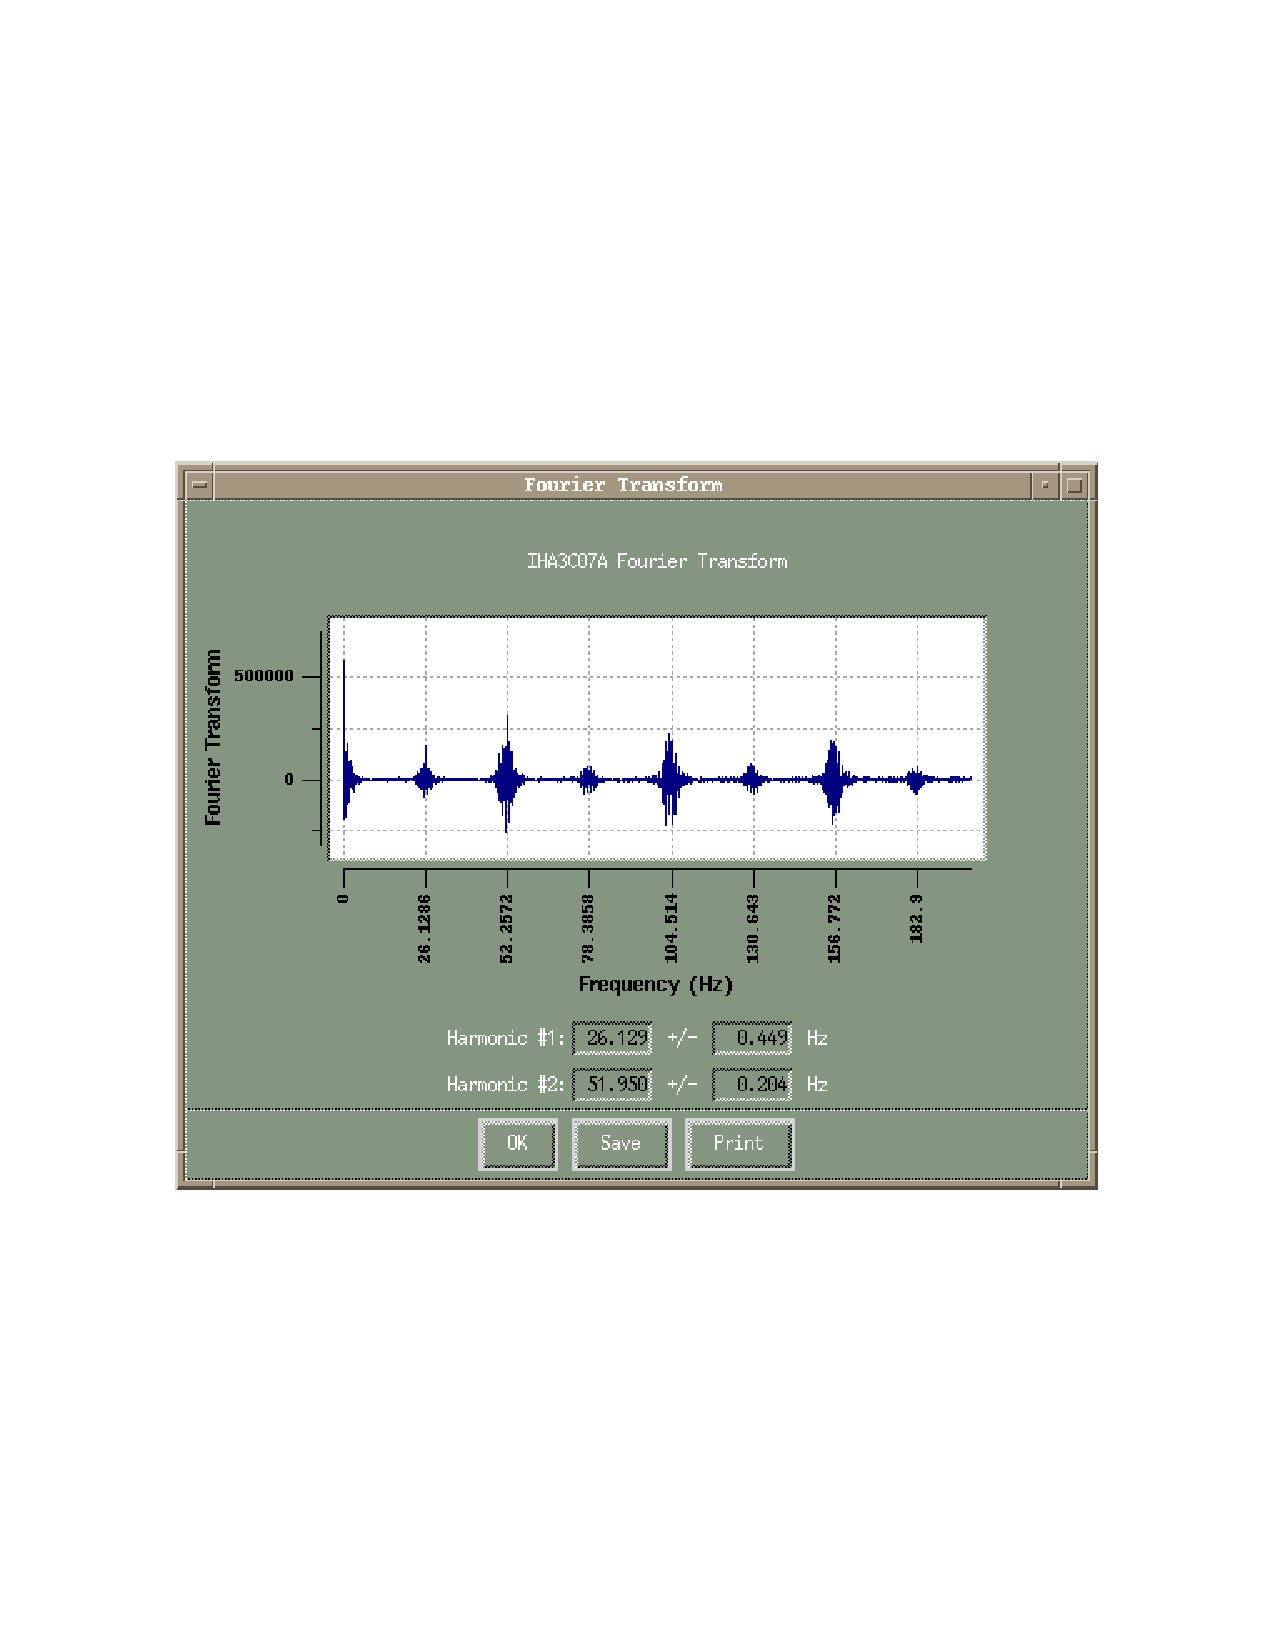
\includegraphics{fourier_transform.pdf}
\caption{The Fourier transform interface.}\label{fig:transform}
\end{figure}
The Fourier transform used to isolate the fundamental frequency of the beam is
\begin{equation}
\hat f(t)=\int_{-\infty}^\infty f(s)\cos \frac{2 \pi s t}{v} {\rm d}x,
\end{equation}
where $v\approx 0.248\mu m/s$ is the speed of the encoder.  Let $N(x)$ be a continuous interpolation of
the harp data, so that $N(x)$ equals the electron count $n_i$ at each of the data points $(x_i, n_i)$ and
0 off the scanning region $(x_{min}, x_{max})$. Then
%\begin{eqnarray}
%\hat N(s)&=&\int_{-\infty}^\infty N(x)\cos \frac{2 \pi s t}{v} {\rm d}x \\
%	&=&\int_{x_{min}}^{x_{max}} N(x)\cos \frac{2 \pi s t}{v} {\rm d}x \\
%	&\approx& \frac{\Delta x}{3}\sum_{i<i_{max}} c_i n_i(x_i) \cos \frac{2 \pi x_i s}{v},
%\end{eqnarray}
%Ed. Note: the above eqnarray was reformatted below for compatibility with latex2html.
\begin{center}
\begin{equation}
\begin{tabular}{rcl}
$\hat N(s)$&$=$&$\int_{-\infty}^\infty N(x)\cos \frac{2 \pi s t}{v} {\rm d}x$ \\
	   &$=$&$\int_{x_{min}}^{x_{max}} N(x)\cos \frac{2 \pi s t}{v} {\rm d}x $\\
	   &$\approx$&$ \frac{\Delta x}{3}\sum_{i<i_{max}} c_i n_i(x_i) \cos \frac{2 \pi x_i s}{v}$,
\end{tabular}
\end{equation}
\end{center}
where $\Delta x=x_{i+1}-x_i,$ $i_{max}$ is an arbitrary large constant, and the $c_i$ are the constants given
by Simpson's integration method.

By Poisson's summation formula, 
\begin{equation}\label{poisson}
\sum_{n=1, 2,\ldots} \hat f(n\omega) =
	\frac{1}{2\omega}\sum_{n=1, 2, \ldots} f\left(\frac{n}{\omega}\right).
\end{equation}
The algorithm used to isolate the fundamental frequency $\omega_0$ of the beam essentially attempts to
maximize the sum (\ref{poisson}).

	\subparagraph{Statistics calculations}

	{\sl Mean and FWHM}

For each superharp scan, the resulting histogram peak centroids are computed using the equation:
%\begin{eqnarray}
%\overline{x}	& = & \frac{\sum \omega_i x_i}{\sum \omega_i}	\\
%\omega_i	& = & \frac{\sqrt{\sum (\Delta n_i)^2}}{n_i} = \frac{\sqrt{\sum n_i}}{n_i} \; ,
%\end{eqnarray}
\begin{center}
\begin{equation}
\begin{tabular}{rcl}
$\overline{x}$&$ = $&$ \frac{\sum \omega_i x_i}{\sum \omega_i}	$\\
$\omega_i    $&$ = $&$ \frac{\sqrt{\sum (\Delta n_i)^2}}{n_i} $\\
              &$ = $&$ \frac{\sqrt{\sum n_i}}{n_i} $\ ,
\end{tabular}
\end{equation}
\end{center}
\noindent
where $n_i$ is the number of counts at the position $x_i$. $\sum n_i$ represents
the total number of events in the selected peak. The beam position is then calculated via:
\begin{equation}
x_{\rm beam} = \overline{x} - x_{\rm survey} \; ,
\end{equation}
where $x_{\rm survey}$ corresponds to the location of each wire if the beam was along the
ideal path inside the beampipe.

The standard deviation (rms) is calculated from the second moment (variance) of the
distribution:
\begin{equation}
M_2 = \sigma^2 =
	\sqrt{\frac{1}{\sum n_i-1}\frac{\sum \omega_i (x_i-\overline{x})^2}{\sum \omega_i}} \; ,
\end{equation}
and the full width at half maximum (FWHM) from:
\begin{equation}
\sigma = \frac{FWHM}{2\sqrt{2ln2}} \; .
\end{equation}

	{\sl Skewness and Kurtosis}

Statistical higher moments $M_n$ are also calculated:
\begin{equation}
M_n = \frac{\sum \omega_i (x_i-\overline{x})^n}{\sum \omega_i} \; , \; {\rm for \; n>2} \; .
\end{equation}
Since the term $1/(\sum n_i-1)$ appears in $\sigma=\sqrt{M_2},$ most statistical calculations
are also normalized.  

The skewness is defined as the measure of the symmetry of a distribution:
\begin{equation}
B_1=\frac{M_3}{M_2^\frac{3}{2}} \; .
\end{equation}
It vanishes for any distribution completely symmetric about its mean (since this forces $M_n$ to 
vanish for odd $n$), and so vanishes for the normal distribution.

The kurtosis is the measure of a distribution's spread about its mean:
\begin{equation}
B_2=\frac{M_4}{M_2^2}-3
\end{equation}
It also vanishes for a normal distribution, since $M_4=3\sigma^2$ and $M_2=\sigma.$

	\subparagraph{Graph Comparisons}

Using survey data, the program isolates the three peaks of the first graph $H_0$ loaded and plots them in the
three lower graph windows.  As subsequent graphs $H_i$ are loaded, the offset
$\overline{x_{H_i}}-\overline{x_{H_0}}$ is calculated over each of those three regions and displayed in the 
upper-right corner of the appropriate graph.  The offsets have the same order and color as the harp names in
the graph legend.
 
When data from both of a pair of harps (e.g. IHA3C17A and IHA3C17B) are loaded, the angle $\theta$ the
beam makes with the horizontal when travelling through the pair is calculated and displayed.  As with the
offsets, the color of the displayed angle matches the color of graph of the harp pair.

\paragraph{Beam energy measurement}\label{energy}

After loading the data from the superharps at the entrance (IHA3C07A and IHA3C07B) and at
the exit (IHA3C17A and IHA3C17B) of the hall C arc beamline, 
the \fbox{Calculate dP/P0} option
will be enabled?  This menu option allows users to calculate the beam incident energy through some
conditions:
\begin{enumerate}
\item If the full width of the first peak of harp IHA3C07A is less than twice the full
width of the first peak of harp IHA3C17A, then the beam is not dispersive enough to perform the
calculation, and an error will be generated.
\item Prior to the calculation, one has to verify the dispersion and the amplification factor at the
exit of the arc related to the hall C beamline optic settings. The default values are now 12.5~cm and 3,
respectively.
\item {\bf Only the MCC operators are allowed to perform the beam energy calculation since there is a setup
procedure to follow~\cite{ebeam_proc99} (see
appendix~\ref{append_ebeam_proc99})}.  The users can
re-evaluate this calculation by asking for the setting current of the arc dipole magnets and loading all
the corresponding superharp data.
\end{enumerate}

The basic idea behind the calculation is as follows.
Suppose a particle with mass $m$ and charge $q$ is subjected to a magnetic field $\vec{B}$ perpendicular
to the plane of the particle's motion, causing it to travel in a circular path of radius $R$. The beam
momentum $P_0$ is determined via:
\begin{equation}
P_0 = \frac{e}{\Theta}\int Bdl
\end{equation}
where $\int Bdl$ is the magnetic field integral over the path of the electron beam and
$\Theta = 34.3^\circ$ is the bending angle through which the electron beam is deflected. $\int Bdl$ is
determined by mapping bending magnets absolutely with a combination of NMR and Hall probes. Taking $e$
as a constant, this leads to the uncertainty relation:
\begin{equation}
\frac{\Delta P}{P_0} = \sqrt{\Big (\frac{\Delta \int Bdl}{\int Bdl}\Big )^{2}
                     + \Big (\frac{\Delta \Theta}{\Theta}\Big )^{2}} \; .
\end{equation}

The inclusion of the beam incident angle is taken into account by utilizing the Lorentz force:
\begin{equation}
\vec{F}=-e\vec{v}\times \vec{B} = m_e\vec{a},
\end{equation}
where $\vec{a}$ is the acceleration and $m_e$ the mass of the electron. Projecting on the three cartesian
axis (z-beam direction, x-transverse horizontal and y-transverse vertical):
\begin{equation}
\left \{
\begin{array}{lll}
a_x & = & -\frac{evB}{m_e} 	\\
a_y & = & 0			\\
a_z & = & 0			\\
\end{array}
\right .
\Leftrightarrow
\left \{
\begin{array}{lll}
v_x & = &  -\frac{evB}{m_e}t + vsin(\theta _x)	\\
v_y & = & vcos(\theta _y)				\\
v_z & = & vcos(\theta _x)				\\
\end{array}
\right .
\end{equation}

\begin{equation}
\Leftrightarrow
\left \{
\begin{array}{lll}\label{eq:txy}
x & = &  -\frac{evB}{2m_e}t^2 + vsin(\theta _x)t + x_0	\\
y & = & vcos(\theta _y)t + y_0				\\
z & = & vcos(\theta _x)t + z_0				\\
\end{array}
\right .
\end{equation}
We are in a case where: $z_0 = 0$. Therefore:
\begin{equation}
\left \{
\begin{array}{lll}
t & = & \frac{z}{vcos(\theta_x)}					\\
x & = & -\frac{eB}{2m_evcos^2(\theta _x)}z^2 + tan(\theta _x)z + x_0	\\
y & = & \frac{cos(\theta _y)}{cos(\theta _x)}z + y_0			\\
\end{array}
\right .
\end{equation}
The system in (\ref{eq:txy}) characterizes the trajectories of the particle along
$x$ and $y$ as a function of its position inside the magnetic region along $z$.

The expression of $x$ represents the trajectory of the particles in the dispersion plane
(where the particles are subject to the magnetic field):
\begin{equation}
x = -\frac{eB}{2Pcos^2(\theta _x)}z^2 + tan(\theta _x)z + x_0,
\end{equation}
where $x = x_{17}$, $x_0 = x_{07}$ and $\theta _x = \theta _{07}$ are determined by using the superharps
at the entrance (IHA3C07) and at the exit (IHA3C17) of the arc. The beam momentum $P$ corrected from
incident beam angle can then be evaluated.

\paragraph{Further Help}

For further assistance, contact
\par
\noindent
\begin{table}[!ht]
\begin{tabular}{l}
Paul Gu\`eye \\
e-mail: {\tt gueye@jlab.org} \\
Phone: (757) 269-7167 \\
Pager: (757) 849-7167 \\
\end{tabular}
\end{table}



}
